\chapter{Результаты исследований}\label{ch:ch1}

      
\section{Сравнительный анализ известных схем}\label{sec:ch1/sec2}
Ниже представлен анализ современных подходов к проблеме повторного обогащения регенерата, а также обрисовываем соответствующий набор методов, основанных на технологии газовой центрифуги и достижениях каскадной теории разделения многокомпонентных смесей.
\subsection{Обоснование ограничений использования ординарных схем}\label{sec:ch1/sec2.1}
Приведен анализ невозможности решить задачу повторного обогащения регенерата в условиях многократного рецикла. Рассмотренный состав, соответствующий пятому рециклу (пятикратному переиспользованию урана в цикле легководного реактора) был проверен на возможность получения свежего НОУ, удовлетворяющего поставленным условиям.

Схемы, одними из первых предложенные для вовлечения урана из ОЯТ в ядерный топливный цикл,основаны на ординарном трехпоточном каскаде \cite{__2012}. Перейдем к их рассмотрению.
\paragraph{Схема с разбавлением на входе}
Рисунки \ref{fig:pre} показывают невозможность использования значительной доли регенерата для получения свежего НОУ требуемых качеств с помощью схемы \ref{fig:diluted_feed}.

\begin{figure}[ht]
  \centerfloat{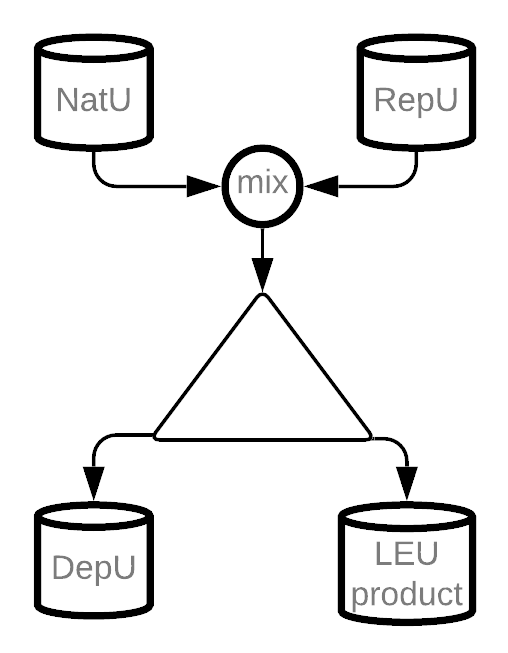
\includegraphics[scale=0.3]{cascades/diluted_feed}}
  \caption{Каскад с разбавлением на входе}\label{fig:diluted_feed}
\end{figure}

\begin{figure}[ht]
  \centerfloat{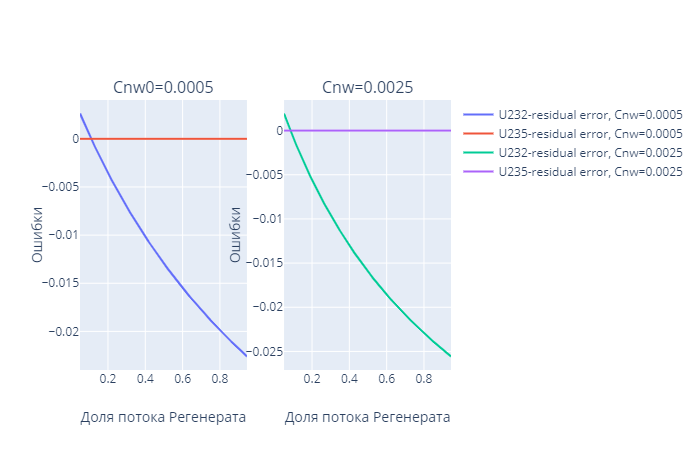
\includegraphics[scale=0.6]{semestr_report/plots/pre}}
  \caption{Зависимость величин ошибок от доли регенерата в потоке питания для различных концентраций $^{235}$U в отвале}\label{fig:pre}
\end{figure}


\paragraph{Схема с разбавлением на выходе}
В такой схеме в начале регенерат обогащают в ординарном каскаде до некоторой концентрации $^{235}$U , которая, очевидно, должна превышать величину 5\%, после чего полученную смесь перемешивают с природным ураном (рисунок \ref{fig:Terminal_Dilution}). Важно отметить, что получаемая смесь должна одновременно соответствовать требуемой величине обогащения по $^{235}$U, а с другой стороны отвечать ограничению по $^{235}$U и удовлетворять условию компенсации $^{236}$U. Таким образом, одновременно должны выполняться 3 условия, однако управляющих параметров в такой задаче только два: выходная концентрация $^{235}$U и соотношение перемешиваемых потоков. При этом важно отметить, что хоть формально выходная концентрация  $^{235}$U и является управляющим параметром, ее изменение неминуемо влечет за собой изменение и
концентраций $^{236}$U и $^{232}$U, тем самым внося неопределенность в решение задачи. Таким
образом, можно констатировать, что, в отличие от случая смешивания обогащенного
природного урана с регенератом, решение для такой каскадной схемы не всегда может
быть найдено, и, по-видимому, зависит от состава регенерата урана.
Так, для состава регенерата пятого рецикла невозможно найти решение, на что указывает анализ русунка \ref{fig:TerminalDilution_results}. Кривые ошибок представляют собой абсолютные отклонения концентраций изотопов $^{235}$U и $^{232}$U в окончательном продукте (после смешивания) от требуемых величин: $^{235}$U с учетом компенсации $^{236}$U и предельно допустимой концентрации $^{232}$U. Таким образом, для данного состава возможно
подобрать только такие параметры каскада, которые будут отвечать либо условию
компенсации  $^{236}$U, либо ограничению на $^{232}$U.

По-видимому, для использования данной схемы необходимо разбавлять обогащенный регенерат не одним разбавителем, а двумя или более. В этом случае при решении задачи появятся дополнительные управляющие параметры, варьирование которых может позволить удовлетворить всем ограничениям
при решение поставленной задачи. Продолжать исследование такой схемы в этом направлении не представляется целесообразным, так как такой подход к повторному обогащению регенерата связан с потерями работы разделения из-за смешения изотопных композиций различных концентраций целевого компонента. Вдобавок, решение подобной задачи, как правило, связано с необходимостью обеспечить условие присутствия регенерата в финальном продукте на заданном соотношении, связанном с формальным условием полного возврата ОЯТ. Такое дополнительное условие влечет необходимость использования еще одного управляющего параметра. К тому же, использование разделительного оборудования только для обогащения грязного `регенерата', когда чистый разбавитель подмешивается независимо (вне каскада газовых центрифуг), не представляется оправданным.

\begin{figure}[ht]
  \centerfloat{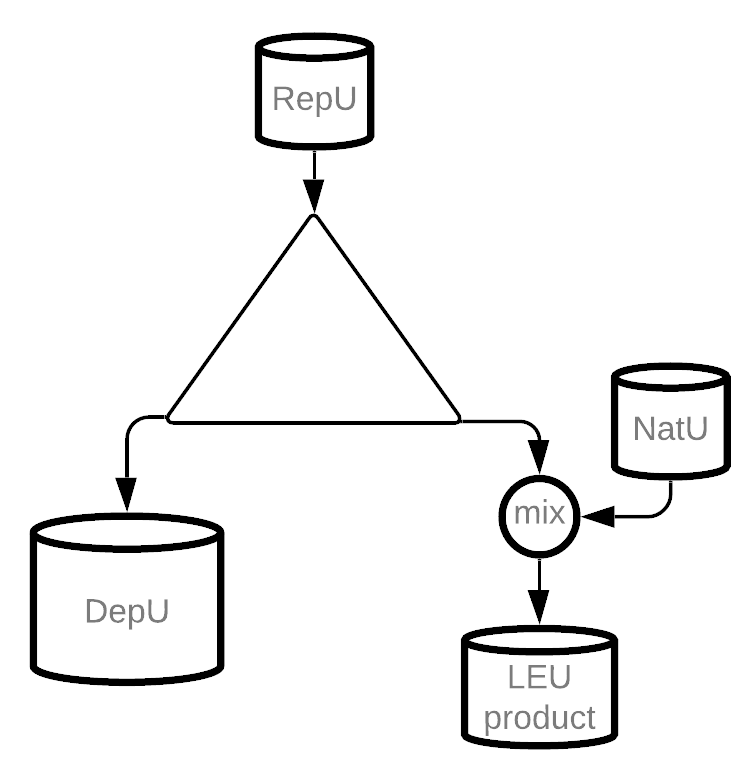
\includegraphics[scale=0.2]{cascades/Terminal_Dilution}}
  \caption{Каскад с разбавлением на выходе}\label{fig:Terminal_Dilution}
\end{figure}

\begin{figure}[ht]
  \centerfloat{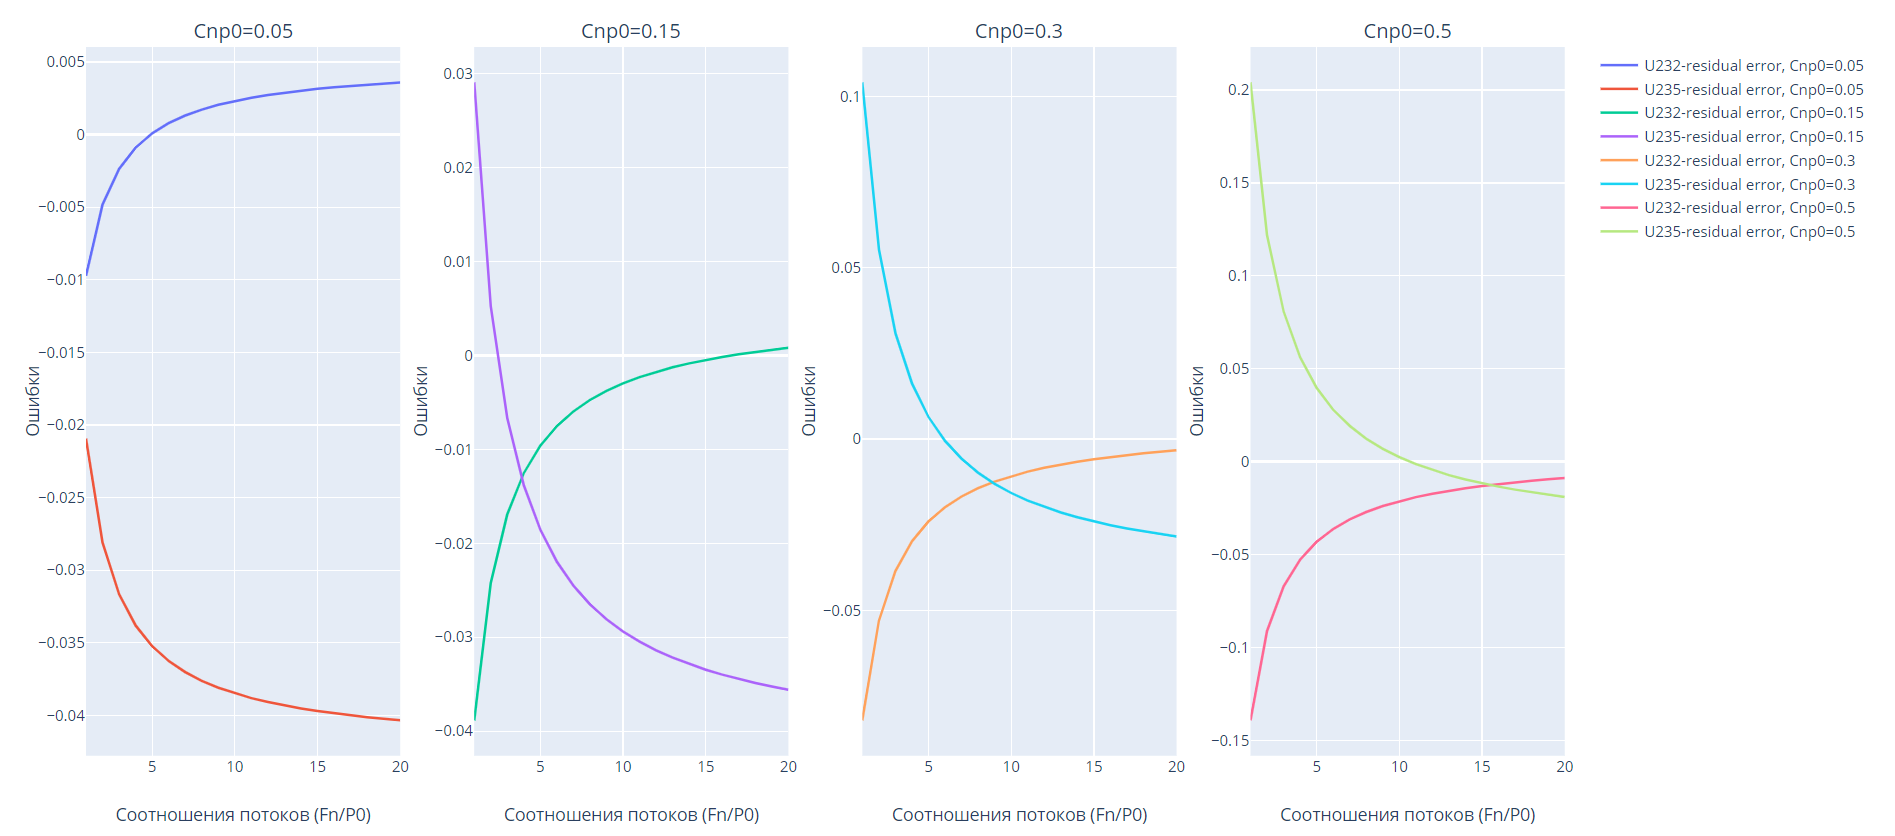
\includegraphics[scale=0.35]{semestr_report/plots/TerminalDilution}}
  \caption{Зависимость величин ошибок от соотношения смешиваемых потоков для различных концентраций  $^{235}$U в обогащенном регенерате}\label{fig:TerminalDilution_results}
\end{figure}


Таким образом, анализ схем на основе базового трехпоточного каскада демонстрирует потребность в модификации компоновок разделительного оборудования в контексте многократного рецикла урана.

Отсюда и вытекает необходимость использовать составные каскадные схемы ввиду необходимости  `пространственного' разделения. Так двойная схема позволяет отделить минорные легкие изотопы $^{232}$U, $^{234}$U в независимом потоке отборной части каскада. Так, например, схема \ref{fig:double} позволяет во втором каскаде разделить потоки, выделив $^{235}$U в тяжелой фракции, направив $^{232}$U и $^{234}$U в легкую.

\begin{figure}[ht]
  \centerfloat{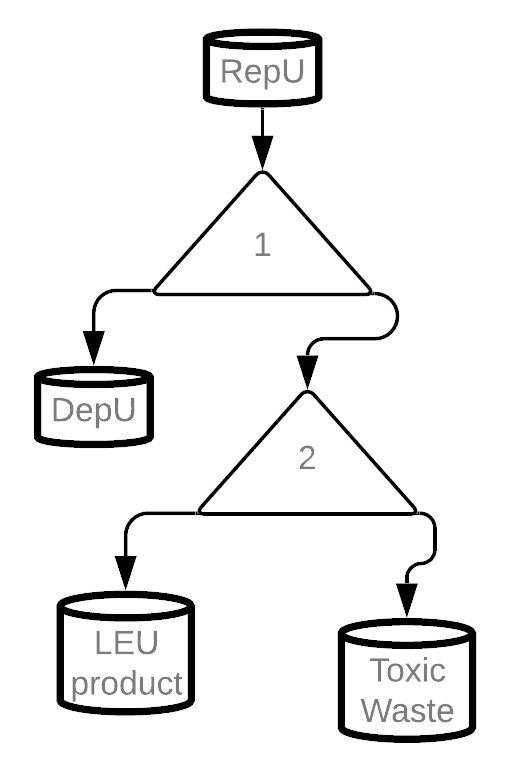
\includegraphics[scale=0.3]{cascades/double}}
  \caption{Двойной каскад}\label{fig:double}
\end{figure}

С появлением свойств такого рода у каскадов, вместо привычной дихотомии, выделяющей схемы с приставкой `много-' (многопоточные схемы, многокаскадные конфигурации), предлагается классифицировать каскады, используемые для обогащения регенерата, как разбавляющие или очищающие. Так, схема двойного каскада является очищающей, в отличие от схем, основанных на ординарном каскаде, работающих на принципе разбавления.  Хоть и любая таксономия арбитрарна, условная граница `касад-разбавитель' -- `каскад-балластоочиститель' гораздо лучше подчеркивает сущностные характеристики анализируемых схем, предназначенных для повторного обогащения урана.

\section{Разработка схем полного возврата}\label{sec:ch2/sec3}
В качестве модификации двойного каскада была предложена альтернативная каскадная схема, которая позволяет обеспечить возврат регенерата в цикл в соотношении 1:1. В этой схеме, изображенной 
на рисунке \ref{fig:vestnik}, первая часть (каскад 1) увеличивает 
концентрацию $^{235}$U со всеми более легкими изотопами ($^{232}$U и $^{234}$U) и направляет их (через выходящий поток в правой части на рисунке) ко второму каскаду, который будет концентрировать эти четные миноры в потоке загрязненного продукта \cite{smirnovObogashchenieRegenerirovannogoUrana2018}.
Хотя на этот раз приготовленная композиция разбавляется НОУ для контроля концентраций $^{232}$U и $^{234}$U в допустимых пределах и для управления соотношением рециклируемых материалов (для поддержания соотношения регенерата в питании каскада к нарабатываемому продукту на уровне 1:1, что формально соответствует полному возврату выгоревшего топлива в ядерный топливный цикл).

\begin{figure}[ht]
  \centerfloat{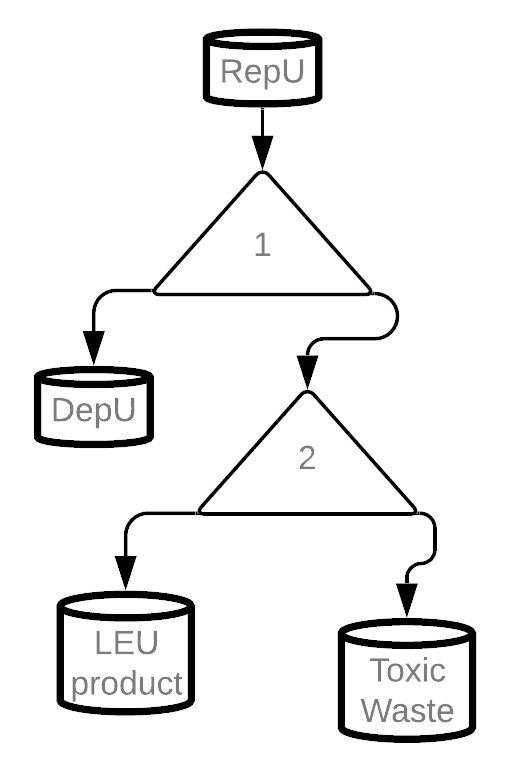
\includegraphics[scale=0.3]{cascades/double}}
  \caption{Двойной каскад с добавлением НОУ (тройной каскад)}\label{fig:vestnik}
\end{figure}

Хотя этот вариант и кажется идеальным, цена хранения побочного продукта из загрязненной смеси слишком высока, что мгновенно делает схему нежизнеспособной, если нет способов избежать такого негативного побочного эффекта.
Однако затем было предложено применить дополнительный каскад для производства НОУ из загрязненной смеси, сильно разбавленной обедненным ураном (которые имеют высокую концентрацию $^{235}$U около $\approx$20\%), чтобы получить конечный продукт в двух исходящих потоках и достичь значительной экономии природного урана ($\approx$38\%) даже для `грязной' композиции, которая уже была пятикратно рециклирована (рисунок \ref{fig:Tomsk}). Расчеты показали, что такой подход позволяет производить НОУ коммерческого качества, расходуя определенное количество переработанного урана и отвечая стандартным спецификациям для  $^{232}$U (и условиям, установленным для других четных изотопов). В то же время, предлагаемая схема обеспечивает большую экономию природного урана, чем большинство схем обогащения переработанного урана. Это могло бы также обеспечить широкомасштабную «мобилизацию» обедненного урана.

\begin{figure}[ht]
  \centerfloat{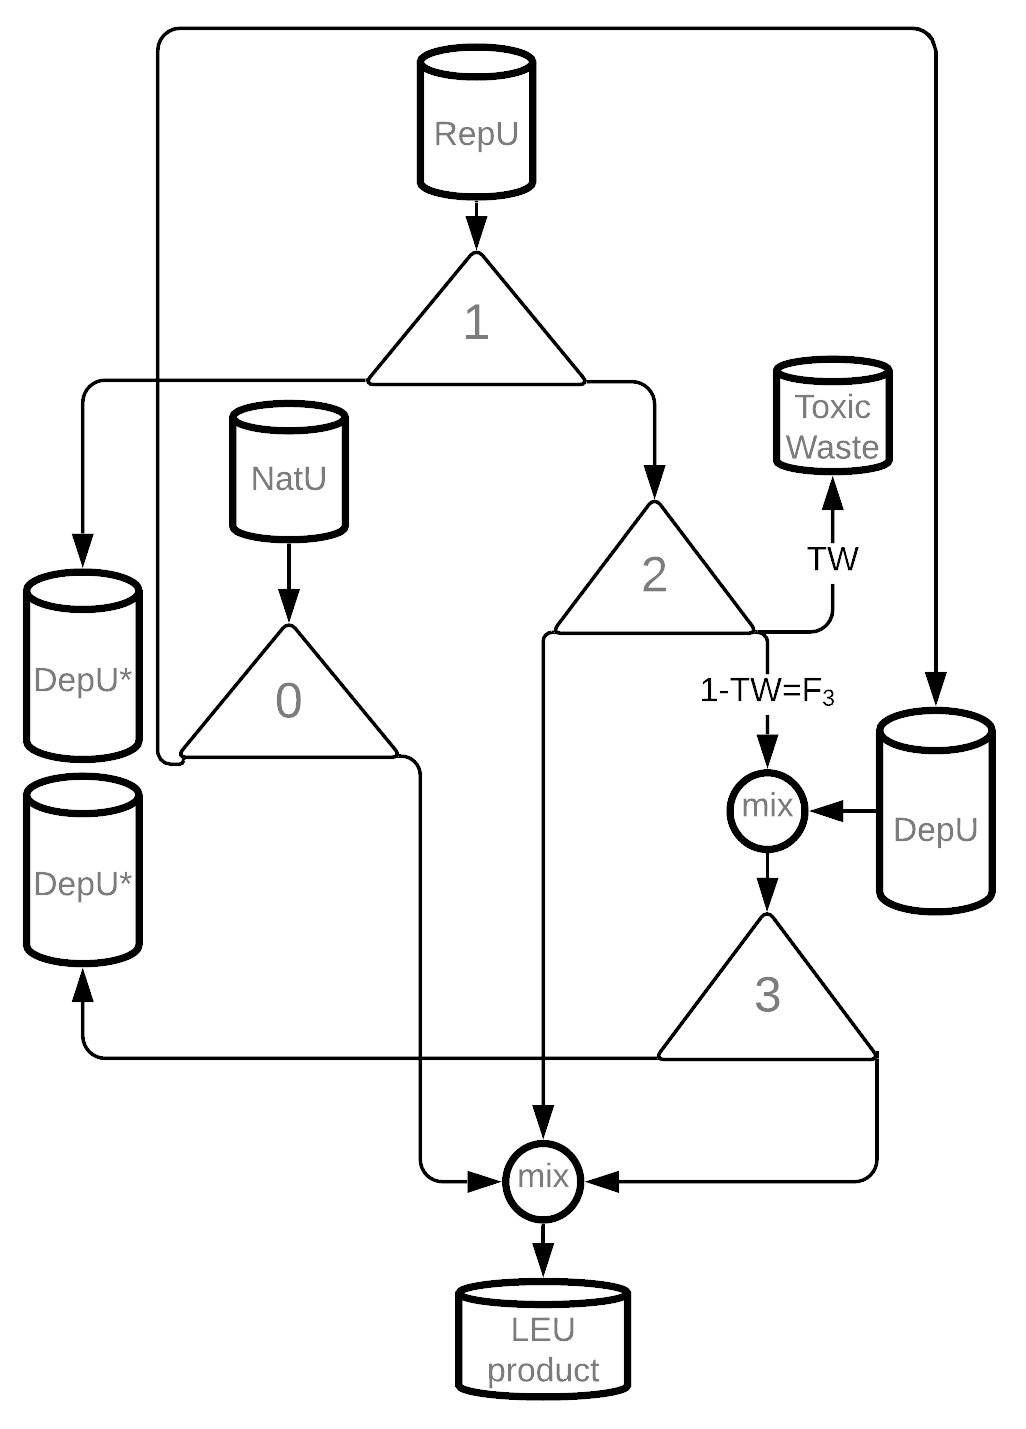
\includegraphics[scale=0.3]{cascades/Triple_Tomsk}}
  \caption{Тройной каскад с подмешиванием ОГФУ и НОУ-разбавителем}\label{fig:Tomsk}
\end{figure}

Затем, в качестве альтернативы была предложена схема рисунка \ref{fig:patent}), в которой на каскад с индексом 3 подается смесь грязного потока легкой фракции каскада 2, которая разбавляется обедненным гексафторидом урана до содержания $^{235}$U на уровне природного урана. Этот поток в дальнейшем разбавляется чистым природным ураном, пропорция которого подбирается для выполнения всех заданных условий.
\begin{figure}[ht]
  \centerfloat{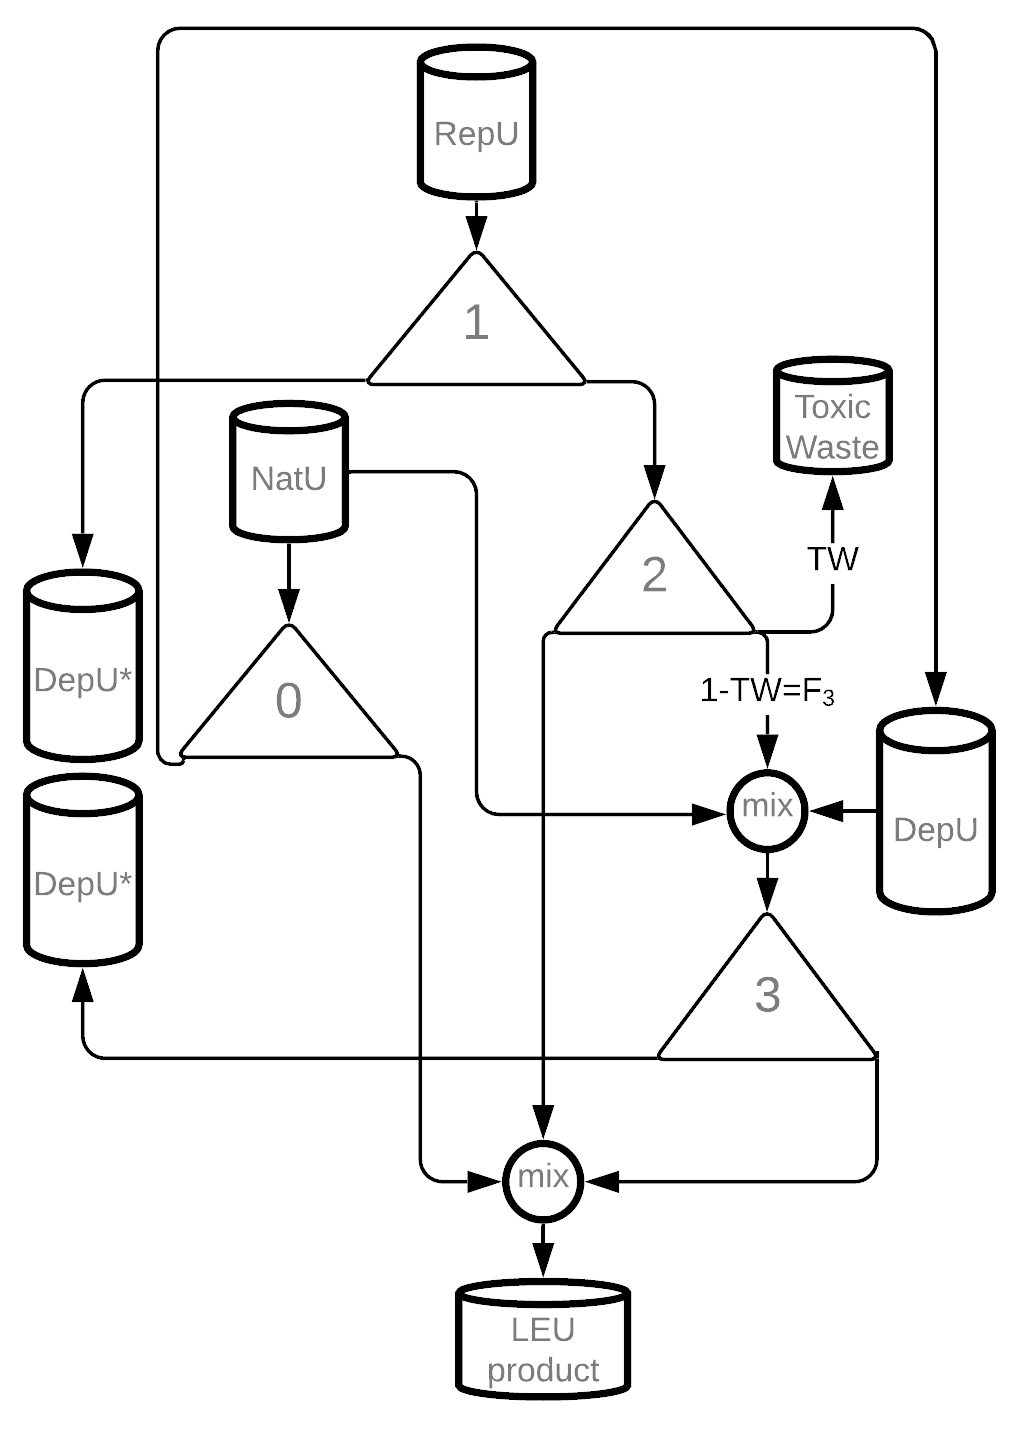
\includegraphics[scale=0.3]{cascades/triple_cascade_complete_return}}
  \caption{Тройной каскад с подмешиванием НОУ, ОГФУ и природного урана}\label{fig:patent}
\end{figure}

Как мы видим, такие схемы также очень ценны как инструмент для переработки всего количества выделенного урана.


\section{Прочие аспекты}\label{sec:ch1/sec1}

Использование регенерированного урана, помимо возможностей расширения ресурсной базы и сокращение отходов, необходимо рассмотреть и с иных позиций. Так, переработка ОЯТ для последующего использования зачастую рассматривается как нежелательная опция с позиций нераспространения ядерного оружия (позиция США в рамках GNEP), а технология газовой центрифуги на сегодня рассматривается экспертами как наиболее чувствительная. То есть, расширение применения двух ключевых технологии для возврата урана в цикл - гидрометаллургического восстановления и газоцентрифужного каскадного обогащения представляется, на первый взгляд, негативным с точки зрения вопроса сдерживания распространения ядерного оружия. Однако, если производство ядерного топлива ограничивается странами - глобальными лидерами в АЭ (как, к примеру, в рамках российской инициативы по созданию системы международных центров по предоставлению услуг ядерного топливного цикла), а неядерным державам, поставляется топливо на основе регенерата урана, ситуация в корне меняется. Благодаря нейтроно-физическим свойствам такого топлива, вариант его переключения представляется гораздо менее осуществимым. Это обусловлено как неизбежным высоким радиационным воздействием в случае операции переключения ядерного материала, сопровождающейся необходимостью его конверсии (несколько стадий) и обогащения, так и легкостью детектирования изъятия даже малых количеств делящегося материала.


\subsection{Ядерное нераспространение. Анализ сценариев переключения}\label{sec:ch1/sec1.1}

Рассмотрен модельный сценарий переключения ядерного материала из топлива легководного реактора типа ВВЭР-1000 или ВВЭР-1200,  изготовленного из регенерированного урана. Предполагали, что АЭС находится под гарантиями МАГАТЭ. Технической целью гарантий является предотвращение или своевременное обнаружение переключения значимого количества ядерных материалов (требования своевременности обнаружения переключения значимого количества ЯМ зависят от  его категории) \cite{bumblis}. Так, в соответствие с \cite{bumblis}, технической целью гарантий МАГАТЭ применительно к реактору ВВЭР-1000 является обнаружение переключения в течение года такого количества низкообогащенного урана, которое содержит более 75 кг $^{235}$U.

В рамках работы рассмотрена модельная задача обнаружения переключения урана из топлива реактора типа ВВЭР со средним обогащением 4,6\%, работающего в полуторагодичном цикле перегрузок. Анализ сценария переключения показал, что технической цели гарантий МАГАТЭ соответствует обнаружение переключения свежих 691 твэла, содержащих 1167,9 кг двуокиси урана или 1029,4 кг урана (включая 75 кг 235U). При перегрузке 72 ТВС из каждой из них может изыматься не более 10 твэлов.

Рассмотрена возможность использования для обогащения переключенного регенерата с помощью:  надкритических центрифуг TC-12 компании URENCO \cite{Borisevich2014}. Для такой центрифуги относительный коэффициент разделения ступени для компонентов 235U и 238U равен 2, а пропускная способность аппарата g взята в интервале 60–80 мг/сек, что соответствует для нее максимальной разделительной мощности. Учитывали, что извлеченное ЗК топливо содержит уран в форме его диоксида, причем подавляющая доля приходится на  $^{238}$U, тогда как ЗК в форме ВОУ будет получено в металлической форме. 

На рисунке \ref{fig:np1} представлена зависимость количества высокообогащенного урана от соотношения концентраций 235U в потоке отвала CW, выраженная в значимых количествах (ЗК). Отметим, что для высокогобогащенного урана (выше 2\%) значимым количеством является всего лишь 25 кг. При этом в выполненных расчетах обогащение материала составляло 90\% (мас.).  Из представленной зависимости видно, что из указанного выше количества переключенного материала всегда можно получить как минимум одно значимое количество ВОУ.
\begin{figure}[ht]
  \centerfloat{
    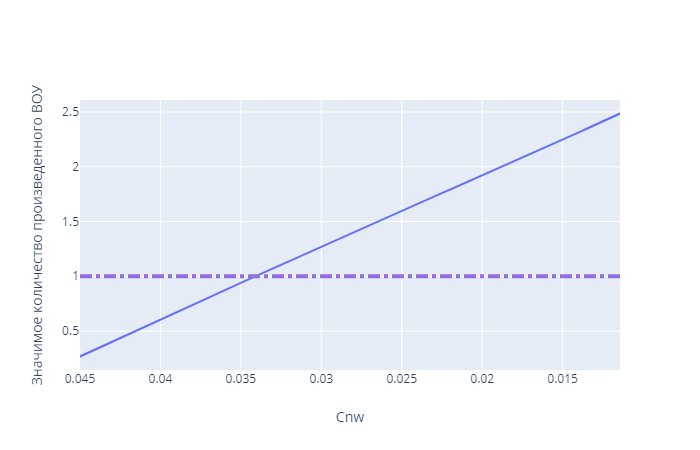
\includegraphics[scale=0.5]{semestr_report/plots/np1}
  }
  \caption{Зависимость количества высокообогащенного урана от степени обеднения по $^{235}$U.}\label{fig:np1}
\end{figure}

\begin{figure}[ht]
  \centerfloat{
    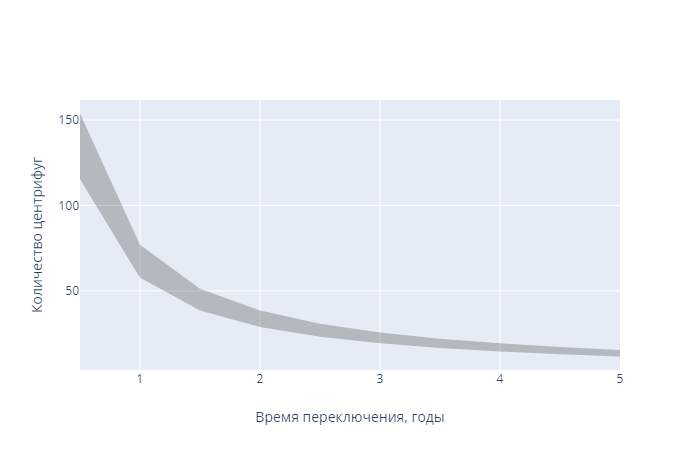
\includegraphics[scale=0.5]{semestr_report/plots/np2}
  }
  \caption{Зависимость количества высокообогащенного урана от степени  обеднения по $^{235}$U.}\label{fig:np2}
\end{figure}

На рисунке \ref{fig:np2} представлена зависимость минимального количества центрифуг для наработки 1 ЗК высокообогащенного урана, от времени.  Из анализа рис. \ref{fig:np2} следует, что имея в качестве исходного материала значимое количество низкообогащенного урана (75 кг), при наличии порядка сотни газовых центрифуг, существует возможность получить значимое количество высокообогащенного урана (25 кг) в срок меньший, чем оцениваемое время переключения, которое составляет порядка 1 года. А при диверсионном необнаруженном переключении, когда последующая проверка не выявляет изъятия топлива, злоумышленники располагают длительными временными периодами, позволяющими получить 1 ЗК ВОУ, располагая всего лишь десятком-другим разделительных аппаратов. Подобный каскад подобного может быть расположен в легко скрываемом лабораторном необъявленном объекте. Важно отметить, что, несмотря на строжайший экспортный контроль, существует возможность приобретения центрифуги на черном рынке или получения скрытой помощи государств, имеющих ядерное оружие или сопутствующие технологии. Заметим также, что такой сценарий гораздо вероятнее для случая переключения НОУ, изготовленного из природного урана, обнаружение извлечения малого количества которого невозможно. 

Подчеркнем, что зависимость на рис. \ref{fig:np2} свидетельствует о том, что 1 ЗК ВОУ, при наличии достаточных разделительных мощностей, может быть произведено до наступления следующей физической инвентаризации (за полгода). Таким образом, приходится признать, что низкообогащенный уран может быть превращен в высокообогащенный за критически короткое время, меньшее, чем интервал между плановыми инспекциями представителей МАГАТЭ. 

Полученные результаты свидетельствуют о том, что оценки работы \cite{rumyanc}, связавшие максимальный риск незаявленного создания ядерного взрывного устройства именно с использованием в качестве стартового материала низкообогащенного урана были  верны. Представленные зависимости наглядно демонстрируют, что период между инспекциями является временем, вполне достаточным для переключения. За рамками работы мы оставили вопрос химической конверсии (превращения оксидов U в фториды U и наоборот (и в металл)) \cite{Orlov2017}, однако это одна из необходимых технологий, требуемых для обогащения урана. 



